\documentclass[11pt,a4paper]{article}
\usepackage[utf8]{inputenc}
\usepackage[T1]{fontenc}
\usepackage{lmodern}
\usepackage[spanish,es-noquoting]{babel}
\usepackage{amsmath,amssymb,bm}
\usepackage{graphicx}
\usepackage{booktabs}
\usepackage{longtable}
\usepackage{tabularx,array}
\usepackage[margin=2.0cm]{geometry}
\usepackage{xcolor}
\usepackage[font=small,labelfont=bf]{caption}
\usepackage{float}
\usepackage[section]{placeins}
\usepackage{microtype}
\usepackage[colorlinks=true,linkcolor=blue!50!black,urlcolor=blue!50!black]{hyperref}
\graphicspath{{fig/}}
\setlength{\parskip}{4pt}
\setlength{\parindent}{0pt}
\newcommand{\code}[1]{\texttt{#1}}
\newcommand{\dd}{\,\mathrm{d}}
\newcommand{\atan}{\operatorname{atan2}}
\newcommand{\dt}[1]{\frac{d}{dt}\!\left(#1\right)}

\title{\vspace{-1.2cm}Segway con patas: manual del modelo\\[4pt]
\large Cinemática, dinámica por Lagrange, dónde está cada cosa en el código y qué parámetros cambiar}
\author{Robótica II, UNCUYO. Generado con Claude Code sobre el repositorio del grupo}
\date{3 de septiembre de 2026}

\begin{document}
\maketitle
\vspace{-0.9cm}

\paragraph{Cómo usar este manual.} Las secciones 1 a 3 definen cada símbolo sobre un esquema y
resuelven la cinemática. Las secciones 4 a 9 deducen la dinámica paso a paso, fila por fila, con
los mismos nombres que usa el código. La sección 10 dice en qué archivo y función está cada
ecuación, y la 11 qué parámetros puede cambiar el ingeniero (masas, inercias, rigideces, fricción,
motor, servo), dónde y con qué unidades. El código es \code{simulacion/planta\_v2/}; el control y
los resultados de simulación quedan para otro informe. Las cotas y masas son del CAD
\code{primera\_iteracion} (medidas sobre el STEP, \code{base\_conocimiento/dimensiones\_cad\_primera\_iteracion.md}).

\section{Notación y convenciones}

\begin{figure}[H]
  \centering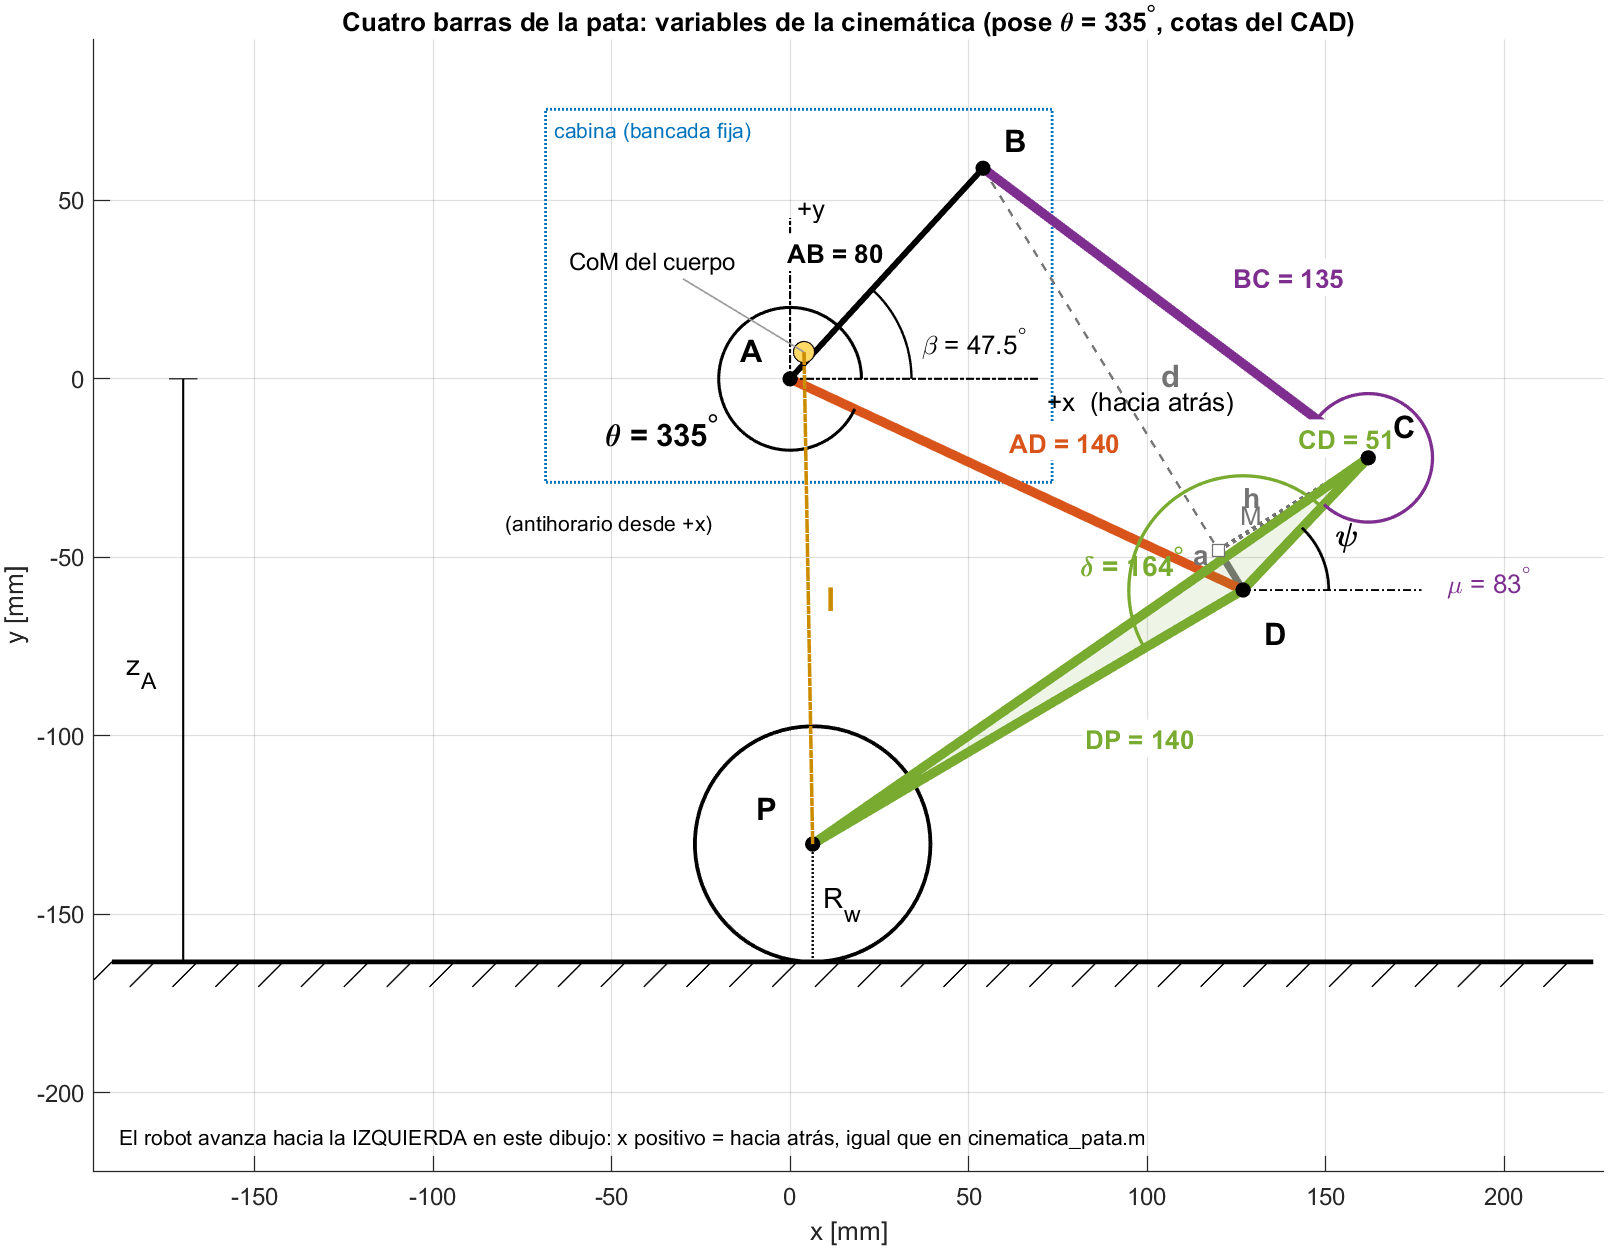
\includegraphics[width=0.98\textwidth]{fig_cinematica_anotada}
  \caption{Variables de la cinemática sobre la geometría real del CAD en la pose $\theta = 335^\circ$.
  Marco cinemático: origen en $A$, $x$ positivo \emph{hacia atrás}, $y$ hacia arriba; el robot avanza
  hacia la izquierda. Los ángulos se miden en sentido antihorario desde $+x$.}
  \label{fig:cin}
\end{figure}

Hay dos marcos y conviene tenerlos separados:
\begin{itemize}\itemsep2pt
  \item \textbf{Marco cinemático} (fig.~\ref{fig:cin}, el de \code{cinematica\_pata.m} del grupo): origen
  en el eje del servo $A$, $x$ hacia atrás, $y$ hacia arriba. Así todos los puntos $C$, $D$ quedan con $x>0$.
  \item \textbf{Marco dinámico} (fig.~\ref{fig:din}): $x$ hacia \emph{adelante} a lo largo del piso, $y$
  normal al piso, como en cualquier péndulo invertido. Pasar de uno a otro es cambiar el signo de $x$;
  las alturas ($y$, $z_A$, $l$) son las mismas.
\end{itemize}

\begin{table}[H]
  \centering\small
  \begin{tabular}{llp{8.6cm}}
    \toprule
    Símbolo & Valor CAD & Significado \\
    \midrule
    $A$, $B$ & $A=(0,0)$; $B = AB(\cos\beta,\sin\beta)$ & pivotes fijos en la cabina: $A$ eje del servo, $B$ pivote del balancín \\
    $AB$, $\beta$ & 80\,mm, 47{,}5° & bancada y su orientación respecto de $+x$ (corregido: 100\,mm, 45°) \\
    $AD$ & 140\,mm & manivela, la mueve el servo \\
    $BC$ & 135\,mm & balancín \\
    $CD$, $DP$, $\delta$ & 51\,mm, 140\,mm, 164° & acoplador: \emph{una} pieza rígida $CDP$; $\delta$ es el ángulo de $D\!\to\!C$ a $D\!\to\!P$ \\
    $\theta$ & 320° a 350° & ángulo de la manivela $A\!\to\!D$ desde $+x$, antihorario. 320° = pata estirada (de pie), 350° = plegada \\
    $\psi$ & sale de la cinemática & ángulo de la dirección $D\!\to\!C$ desde $+x$ \\
    $\mu_t$ & 60° a 90° & ángulo de transmisión en $C$, entre $C\!\to\!D$ y $C\!\to\!B$ (no confundir con la fricción $\mu$) \\
    $\rho$ & $+1$ & rama de armado (de qué lado de la recta $BD$ queda $C$) \\
    $d, a, h, M$ & construcción & $d = |B-D|$; $M$ pie de la perpendicular desde $C$ a $BD$; $a = |D-M|$, $h = |C-M|$ \\
    $P$, $R$ & 33\,mm & eje de rueda y radio de rueda \\
    $z_A$ & 108 a 212\,mm & altura de $A$ sobre el piso: $z_A = R - P_y$ \\
    $\mathrm{CoM}$ & (3{,}9 atrás, 7{,}5 arriba) mm & centro de masa del cuerpo suspendido, respecto de $A$ \\
    $l$ & 83 a 186\,mm & distancia del eje de rueda al CoM: el largo del péndulo \\
    $G$ & 0{,}20\,m/rad & $|\dd l/\dd\theta|$, ganancia del mecanismo \\
    \midrule
    $x$, $y$ & & posición del eje de rueda: a lo largo del piso y en altura sobre el primer descanso \\
    $\phi$ & & ángulo de la recta eje$\to$CoM desde la normal al piso (+ adelante) \\
    $\alpha$ & & pendiente del piso (+ subida hacia adelante); la IMU mide $\phi+\alpha$ \\
    $m_b$, $J_b$ & 0{,}78\,kg, $2{,}8\cdot10^{-3}$\,kg\,m$^2$ & masa e inercia (respecto de su CoM) del cuerpo suspendido \\
    $m_w$, $J_w$ & 0{,}25\,kg, $1{,}6\cdot10^{-5}$\,kg\,m$^2$ & masa en el eje (2 ruedas + 2 motores) e inercia de una rueda \\
    $\theta_w$, $\omega$ & & giro y velocidad de cada rueda (+ = rodar hacia adelante) \\
    $\theta_m$, $\omega_m$, $i$ & & giro, velocidad y corriente del rotor de cada motor \\
    $n_g$, $J_r$ & 100 (CAD) ó 21{,}3; $6\cdot10^{-7}$\,kg\,m$^2$ & relación del reductor e inercia del rotor \\
    $\tau_g$, $f$, $N$ & & par del reductor sobre la rueda; fuerza de piso tangencial; normal \\
    $\delta$, $\hat n$, $\hat t$ & & penetración de la rueda en el piso, normal y tangente del contacto \\
    $\tau_s$, $n_s$, $F_l$ & $n_s = 2$ & par de cada servo, cantidad de servos, fuerza equivalente a lo largo de la pata \\
    $l_m$, $s_c$ & & largo que impone el cuatro barras y compresión del flexor $s_c = l_m - l$ (sólo con flexor) \\
    $F_x$, $M_p$, $F_{esc}$ & & perturbaciones: fuerza en el CoM, momento de cabeceo, golpe horizontal en el eje \\
    \bottomrule
  \end{tabular}
  \caption{Símbolos. Valores del CAD tal como está (variante \code{cad}).}
  \label{tab:simb}
\end{table}

\section{Cinemática directa: de $\theta$ a $D$, $C$ y $P$}

Se conoce $\theta$ y se buscan los tres puntos móviles (fig.~\ref{fig:cin}).

\begin{enumerate}\itemsep3pt
  \item \textbf{Manivela.} $D$ gira alrededor de $A$:
  \begin{equation}
    D = A + AD\,(\cos\theta,\ \sin\theta).
    \label{eq:D}
  \end{equation}
  \item \textbf{Acoplador por intersección de circunferencias.} $C$ está a distancia $BC$ de $B$ y a
  distancia $CD$ de $D$. Con $\bm v = B - D$, $d = |\bm v|$, el pie de la perpendicular $M$ queda a
  distancia $a$ de $D$ sobre $DB$ y $C$ a distancia $h$ de $M$ en dirección perpendicular:
  \begin{equation}
    a = \frac{CD^2 - BC^2 + d^2}{2d}, \qquad h = \sqrt{CD^2 - a^2}, \qquad
    M = D + a\,\frac{\bm v}{d}, \qquad C = M + \rho\, h\,\frac{(v_y,\,-v_x)}{d}.
    \label{eq:C}
  \end{equation}
  La fórmula de $a$ sale de restar las dos ecuaciones de circunferencia $a^2 + h^2 = CD^2$ y
  $(d-a)^2 + h^2 = BC^2$. El signo $\rho$ elige una de las dos soluciones; $\rho = +1$ es la rama del
  CAD ($C$ del lado de $x$ mayor). El mecanismo cierra sólo si $|BC - CD| < d < BC + CD$.
  \item \textbf{Punto de rueda.} $P$ es solidario al acoplador: se gira $\delta$ desde $D\!\to\!C$ y se
  avanza $DP$:
  \begin{equation}
    \psi = \atan(C_y - D_y,\ C_x - D_x), \qquad P = D + DP\,\big(\cos(\psi+\delta),\ \sin(\psi+\delta)\big).
    \label{eq:P}
  \end{equation}
  Con $\delta = 164^\circ$, $P$ queda casi en la prolongación de $C\!\to\!D$ (el plano acota el
  suplementario, 16°: no cargar 16 donde va 164).
  \item \textbf{Ángulo de transmisión.} $\cos\mu_t' = \dfrac{(D-C)\cdot(B-C)}{|D-C|\,|B-C|}$,
  $\mu_t = \min(\mu_t',\ \pi - \mu_t')$. Cerca de 0° ó 180° el mecanismo se traba; en el CAD va de 60° a 90°.
\end{enumerate}

Es la misma construcción que la deducción a mano del grupo (\code{modelado/cinematica/geometrico\_1.jpeg}):
allí $\cos\beta_{BD} = (BC^2 + d^2 - CD^2)/(2\,BC\,d)$ desde $B$, que es $BC\cos\beta_{BD} = d - a$.
Las diferencias son de marco ($B$ sobre el eje $x$ y barras como múltiplos de $L$), no de método.

\textbf{Alturas y largo del péndulo.} El piso está a $R$ por debajo de $P$:
\begin{equation}
  z_A = R - P_y, \qquad h_{tapa} = z_A + 0{,}0745, \qquad l = -P_y + y_{\mathrm{CoM}} .
  \label{eq:l}
\end{equation}
$l$ es la única salida de la cinemática que usa la dinámica. El desvío horizontal de $P$ respecto de la
vertical de $A$ no entra en $l$: $\phi$ es el ángulo de la recta $P\!\to\!\mathrm{CoM}$, así que ese desvío
se absorbe como una inclinación pequeña de la cabina en equilibrio (hasta 4° en el CAD actual).

\begin{figure}[H]
  \centering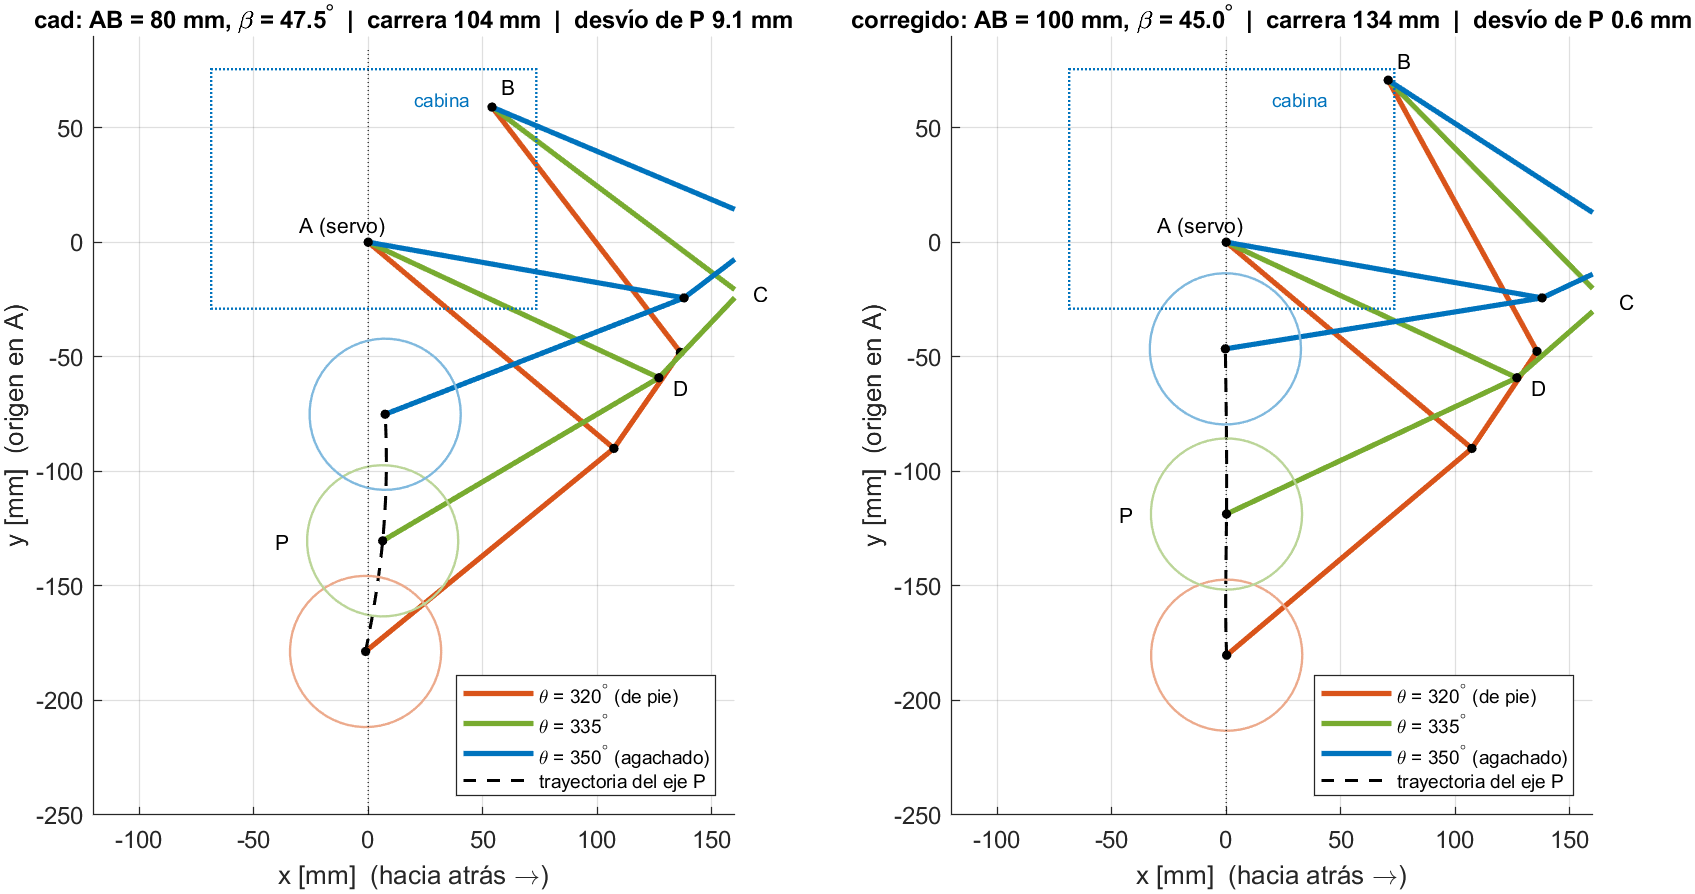
\includegraphics[width=\textwidth]{fig_mecanismo}
  \caption{Tres poses y trayectoria de $P$. Izquierda: CAD tal como está (bancada 80\,mm con barras de
  escala 100). Derecha: bancada a 100\,mm a 45°, la escala para la que se diseñaron las barras.}
  \label{fig:mec}
\end{figure}

\begin{table}[H]
  \centering\small
  \begin{tabular}{lrr}
    \toprule
     & CAD (AB = 80\,mm, $\beta$ = 47{,}5°) & corregido (AB = 100\,mm, $\beta$ = 45°) \\
    \midrule
    Carrera de $P$ entre 320° y 350° & 103{,}5\,mm & 133{,}7\,mm \\
    Desvío horizontal de $P$ & 9{,}1\,mm (8{,}7\,\%) & 0{,}6\,mm (0{,}4\,\%) \\
    Tope de la tapa de pie / agachado & 286 / 182\,mm & 288 / 154\,mm \\
    $\mu_t$ mínimo & 60° & 58° \\
    Rango de $l$ & 83 a 186\,mm & 54 a 188\,mm \\
    \bottomrule
  \end{tabular}
  \caption{Cinemática directa evaluada en el recorrido del servo.}
\end{table}

\section{Cinemática inversa: de $l$ (o de la altura) a $\theta$}

$\theta(l)$ no tiene expresión cerrada ($P$ depende de $\theta$ a través de la raíz de \eqref{eq:C}), pero
$l(\theta)$ es monótona en el recorrido, así que la inversa es única y se resuelve por tabla:
\code{parametros\_robot} evalúa \eqref{eq:D}--\eqref{eq:l} en 121 valores de $\theta$ y guarda 21 nodos
equiespaciados en $l$ con $\theta(l)$ y $\dd\theta/\dd l$ (fig.~\ref{fig:mapa}); \code{interp\_lin}
interpola. Como cualquier altura se convierte en $l$ con \eqref{eq:l}, la misma tabla resuelve
``qué $\theta$ hace falta para tal altura''. No tiene sentido pedir $\theta$ para un $(x,y)$
arbitrario: $P$ tiene un solo grado de libertad y sólo recorre la curva de la figura~\ref{fig:mec}.

\begin{figure}[H]
  \centering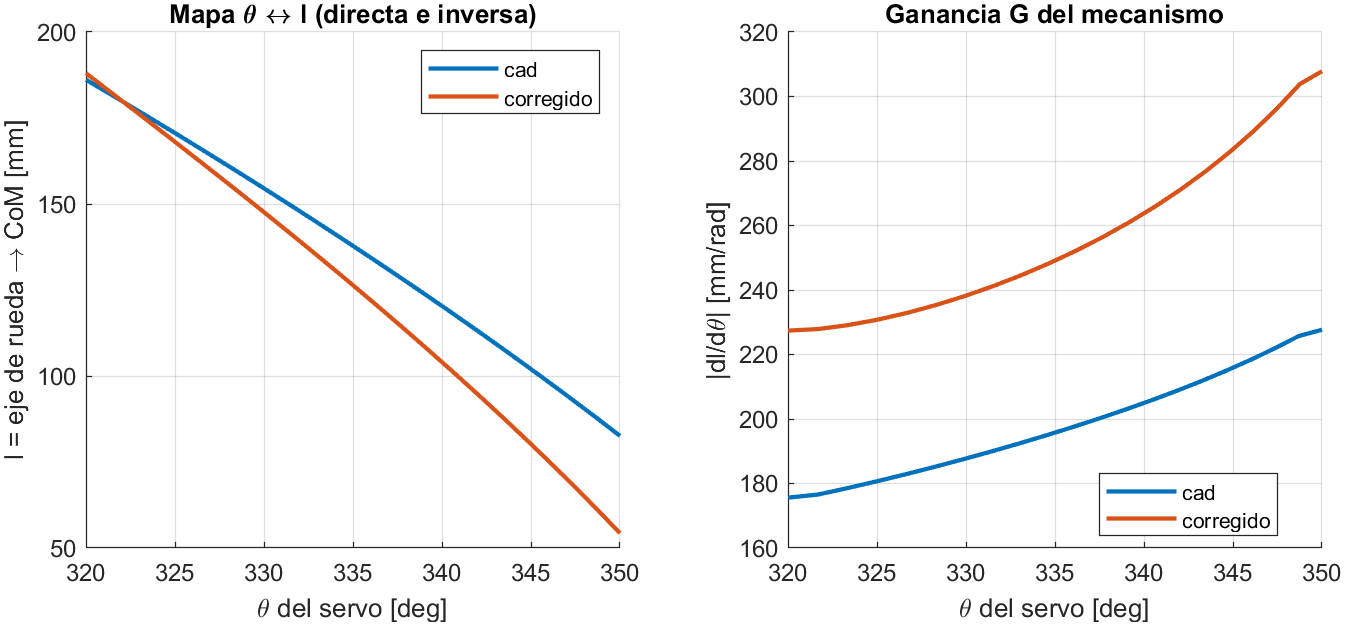
\includegraphics[width=0.95\textwidth]{fig_mapa_theta_l}
  \caption{Izquierda: $l(\theta)$, se lee en cualquier sentido. Derecha: ganancia $G = |\dd l/\dd\theta|$.}
  \label{fig:mapa}
\end{figure}

\textbf{Velocidades y fuerzas.} $\dot l = (\dd l/\dd\theta)\,\dot\theta$. Por trabajo virtual, un par en el
hombro equivale a una fuerza a lo largo del péndulo:
\begin{equation}
  \tau_s\,\delta\theta = F\,\delta l \ \Rightarrow\ F_l = n_s\,\tau_s\,\frac{\dd\theta}{\dd l},
  \qquad \frac{\dd\theta}{\dd l} < 0 \text{ en esta geometría}.
  \label{eq:tv}
\end{equation}
Sostener el peso del cuerpo ($m_b g = 7{,}7$\,N) cuesta $m_b g\,G/n_s = 0{,}76$\,N\,m por servo en el
CAD (0{,}99 en el corregido, que tiene más carrera); el DS3225MG da 2{,}4.

\section{Dinámica del cuerpo por Lagrange}

\subsection{Hipótesis}
\begin{enumerate}\itemsep2pt
  \item Movimiento en el plano sagital; las dos patas sincronizadas (mismo $\theta$); los dos motores
  suman su par; sin guiñada.
  \item El cuerpo suspendido (cabina, tapa, servos, batería, electrónica, barras) es un rígido de masa
  $m_b$ e inercia $J_b$ con su CoM a distancia $l$ del eje de rueda. Las barras se mueven con $\theta$;
  su aporte al CoM y a $J_b$ se promedia sobre el recorrido. El cambio de $l$ es un grado de libertad
  prismático.
  \item Ruedas y motores ($m_w$) están en el eje. El eje puede subir y bajar ($y$): el robot puede
  despegar y caer.
  \item La rueda no rueda por definición: su giro es un estado propio y la fuerza de piso sale de un
  modelo de contacto (sección~\ref{sec:contacto}).
  \item El piso puede tener pendiente $\alpha$ (se rota la gravedad) y escalones (perfil).
  \item El servo es una fuente de par con lazo interno y entra por \eqref{eq:tv}; la inercia del cuatro
  barras alrededor del hombro se desprecia.
\end{enumerate}

\begin{figure}[H]
  \centering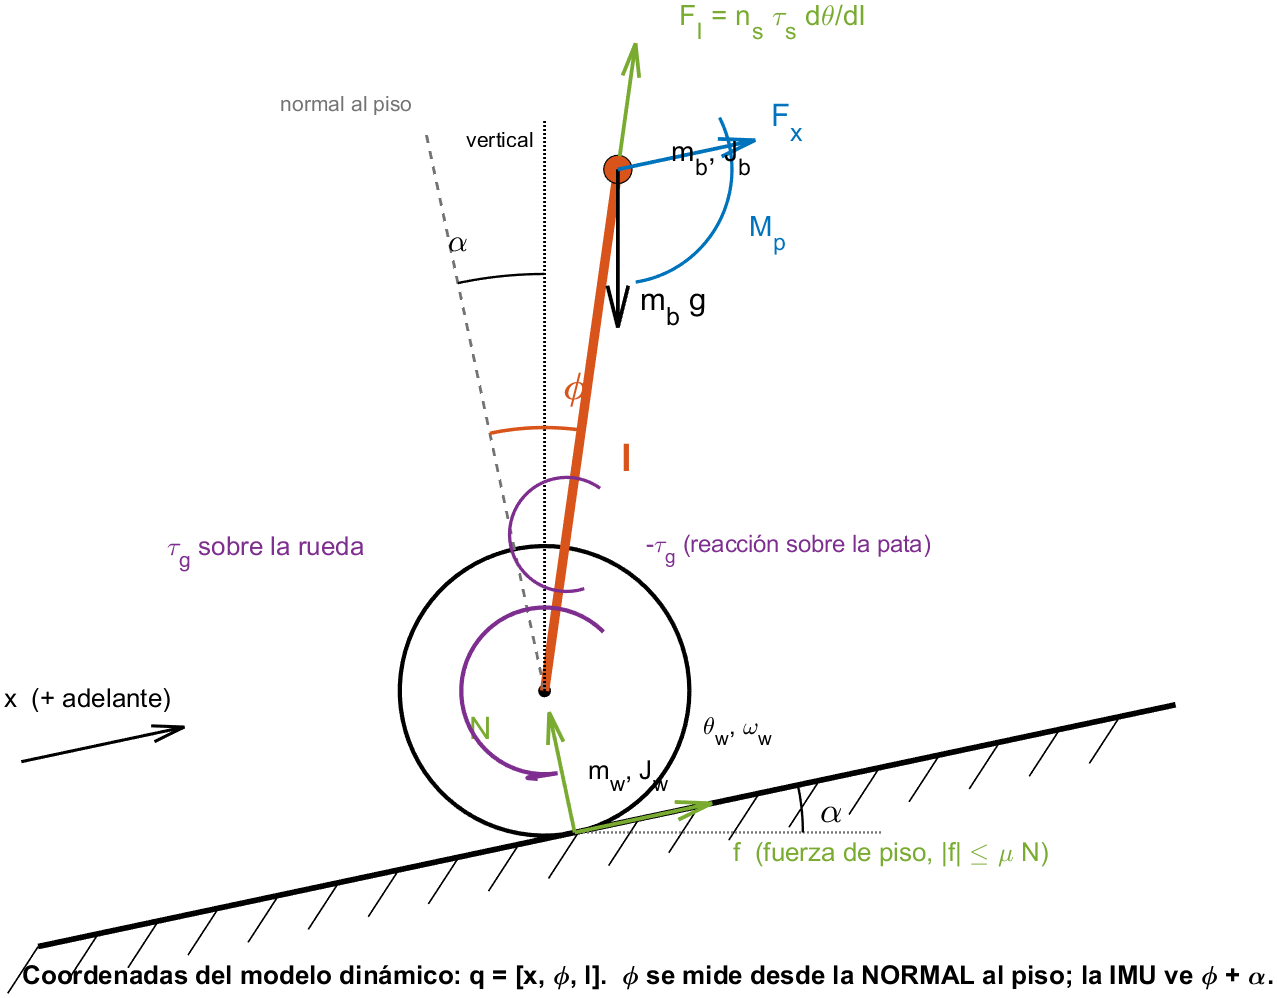
\includegraphics[width=0.78\textwidth]{fig_dinamica}
  \caption{Coordenadas generalizadas $q = [x, y, \phi, l]$ y fuerzas que entran en las ecuaciones,
  sobre un piso con pendiente $\alpha$. $\phi$ se mide desde la normal al piso, hacia adelante.}
  \label{fig:din}
\end{figure}

\subsection{Posiciones, velocidades y energías}

En el marco del piso, con $c = \cos\phi$ y $s = \sin\phi$:
\begin{equation}
  \bm r_w = (x,\ y), \qquad \bm r_b = (x + l\,s,\ y + l\,c), \qquad
  \dot{\bm r}_b = \big(\dot x + \dot l\,s + l\dot\phi\,c,\ \ \dot y + \dot l\,c - l\dot\phi\,s\big).
\end{equation}
Energía cinética: masa del eje + traslación del CoM + rotación del cuerpo. Al expandir $|\dot{\bm r}_b|^2$
los productos cruzados $\dot l\,s\cdot l\dot\phi\,c$ y $\dot l\,c\cdot l\dot\phi\,s$ se cancelan:
\begin{equation}
  T = \tfrac12 (m_w + m_b)(\dot x^2 + \dot y^2) + \tfrac12 m_b(\dot l^2 + l^2\dot\phi^2)
      + m_b\,\dot x(\dot l\,s + l\dot\phi\,c) + m_b\,\dot y(\dot l\,c - l\dot\phi\,s) + \tfrac12 J_b\dot\phi^2 .
  \label{eq:T}
\end{equation}
Energía potencial con la gravedad rotada por la pendiente, $\bm g = g(-\sin\alpha, -\cos\alpha)$:
\begin{equation}
  V = -m_b\,\bm g\cdot\bm r_b - m_w\,\bm g\cdot\bm r_w
    = (m_b + m_w)\,g\,(x\sin\alpha + y\cos\alpha) + m_b\,g\,l\cos(\phi - \alpha).
  \label{eq:V}
\end{equation}
El Lagrangiano es $L = T - V$ y las ecuaciones de Euler--Lagrange con fuerzas generalizadas $Q_i$:
\begin{equation}
  \dt{\frac{\partial T}{\partial\dot q_i}} - \frac{\partial T}{\partial q_i} + \frac{\partial V}{\partial q_i} = Q_i,
  \qquad q = [x,\ y,\ \phi,\ l].
  \label{eq:EL}
\end{equation}

\subsection{Deducción fila por fila}

\textbf{Fila $x$.} De \eqref{eq:T}, $\partial T/\partial\dot x = (m_w+m_b)\dot x + m_b(\dot l\,s + l\dot\phi\,c)$.
Derivando en el tiempo (recordar que $s$, $c$ y $l$ dependen de $t$):
\begin{equation}
  \dt{\frac{\partial T}{\partial\dot x}} = (m_w+m_b)\ddot x + m_b\,s\,\ddot l + m_b\,l\,c\,\ddot\phi
  + m_b\big(2\dot l\dot\phi\,c - l\dot\phi^2 s\big).
\end{equation}
$\partial T/\partial x = 0$ y $\partial V/\partial x = (m_b+m_w)g\sin\alpha$. Los tres primeros términos son la
fila 1 de $M\ddot q$; el paréntesis es $C_1$; la gravedad es $G_{v,1}$.

\textbf{Fila $y$.} $\partial T/\partial\dot y = (m_w+m_b)\dot y + m_b(\dot l\,c - l\dot\phi\,s)$, y
\begin{equation}
  \dt{\frac{\partial T}{\partial\dot y}} = (m_w+m_b)\ddot y + m_b\,c\,\ddot l - m_b\,l\,s\,\ddot\phi
  - m_b\big(2\dot l\dot\phi\,s + l\dot\phi^2 c\big), \qquad \frac{\partial V}{\partial y} = (m_b+m_w)g\cos\alpha .
\end{equation}

\textbf{Fila $\phi$.} $\partial T/\partial\dot\phi = (J_b + m_b l^2)\dot\phi + m_b l(\dot x\,c - \dot y\,s)$.
Su derivada temporal contiene, además de los términos en $\ddot q$, el grupo
$m_b(\dot x\dot l\,c - \dot x l\dot\phi\,s - \dot y\dot l\,s - \dot y l\dot\phi\,c)$; y
$\partial T/\partial\phi = m_b\dot x(\dot l\,c - l\dot\phi\,s) - m_b\dot y(\dot l\,s + l\dot\phi\,c)$ es exactamente
ese mismo grupo, así que se cancelan. Queda
\begin{equation}
  (J_b + m_b l^2)\ddot\phi + m_b l\,c\,\ddot x - m_b l\,s\,\ddot y + 2 m_b l\dot l\dot\phi
  + \frac{\partial V}{\partial\phi} = Q_\phi, \qquad \frac{\partial V}{\partial\phi} = -m_b g l\sin(\phi-\alpha) = m_b g l\sin(\alpha-\phi).
\end{equation}
Con $\alpha = 0$ es $-m_b g l\sin\phi$: el par de vuelco del péndulo invertido, negativo porque inclinarse
hacia adelante hace caer hacia adelante.

\textbf{Fila $l$.} $\partial T/\partial\dot l = m_b\dot l + m_b(\dot x\,s + \dot y\,c)$;
$\dt{\cdot} = m_b\ddot l + m_b s\ddot x + m_b c\ddot y + m_b\dot\phi(\dot x c - \dot y s)$;
$\partial T/\partial l = m_b l\dot\phi^2 + m_b\dot\phi(\dot x c - \dot y s)$. Otra vez los términos con
$\dot x$, $\dot y$ se cancelan y queda
\begin{equation}
  m_b\ddot l + m_b s\,\ddot x + m_b c\,\ddot y - m_b l\dot\phi^2 + m_b g\cos(\phi - \alpha) = Q_l .
\end{equation}
$-m_b l\dot\phi^2$ es la fuerza centrífuga que tiende a estirar la pata; $m_b g\cos\phi$ es el peso que la
pata sostiene.

\subsection{Forma matricial}

Juntando las cuatro filas:
\begin{equation}
  M(q)\,\ddot q + C(q,\dot q) + G_v(q) = Q,
  \label{eq:lag}
\end{equation}
\begin{equation}\small
  M = \begin{bmatrix} m_b+m_w & 0 & m_b l c & m_b s \\ 0 & m_b+m_w & -m_b l s & m_b c \\ m_b l c & -m_b l s & J_b + m_b l^2 & 0 \\ m_b s & m_b c & 0 & m_b \end{bmatrix},\quad
  C = \begin{bmatrix} m_b\dot\phi\,(2\dot l c - l\dot\phi s) \\ -m_b\dot\phi\,(2\dot l s + l\dot\phi c) \\ 2 m_b l\dot l\dot\phi \\ -m_b l\dot\phi^2 \end{bmatrix},\quad
  G_v = \begin{bmatrix} (m_b+m_w)g\sin\alpha \\ (m_b+m_w)g\cos\alpha \\ m_b g l\sin(\alpha-\phi) \\ m_b g\cos(\alpha-\phi) \end{bmatrix}.
\end{equation}
$M$ es simétrica y definida positiva (es la matriz de masa). En el código no se escribió a mano: el
Symbolic Math Toolbox arma \eqref{eq:T}, \eqref{eq:V}, calcula $M = \partial^2 T/\partial\dot q^2$,
$C$ por símbolos de Christoffel, $C_i = \sum_{j,k}\tfrac12(\partial_k M_{ij} + \partial_j M_{ik} - \partial_i M_{jk})\dot q_j\dot q_k$,
y $G_v = \partial V/\partial q$, y genera \code{dinamica\_cuerpo\_gen.m}. La deducción a mano de arriba
sirve para revisarlo. Dos chequeos que están en los tests: quitando la fila y columna de $y$ se
recupera el modelo plano de \code{dinamica\_sl.m} del zip del grupo, y en reposo sobre el piso
todas las aceleraciones dan cero.

\section{Fuerzas generalizadas por trabajo virtual}
\label{sec:Q}

Una fuerza $\bm F$ aplicada en un punto $\bm r(q)$ y un par $\tau$ que actúa sobre una coordenada
angular hacen trabajo virtual $\delta W = \bm F\cdot\delta\bm r + \tau\,\delta\phi$, y como
$\delta\bm r = \sum_i (\partial\bm r/\partial q_i)\,\delta q_i$, la fuerza generalizada es
$Q_i = \bm F\cdot\partial\bm r/\partial q_i$. Para el eje y el CoM:
\begin{equation}
  \frac{\partial\bm r_w}{\partial q} = \big[(1,0),\ (0,1),\ (0,0),\ (0,0)\big], \qquad
  \frac{\partial\bm r_b}{\partial q} = \big[(1,0),\ (0,1),\ (l c, -l s),\ (s, c)\big].
\end{equation}

\begin{itemize}\itemsep3pt
  \item \textbf{Fuerza de contacto} $(F_{cx}, F_{cy})$ aplicada en el eje (sección~\ref{sec:contacto}):
  $Q_x \mathrel{+}= F_{cx}$, $Q_y \mathrel{+}= F_{cy}$. No entra en $\phi$ ni en $l$ porque el eje no depende de ellas.
  \item \textbf{Reacción del motor.} El reductor aplica $\tau_g$ a la rueda; el estator y la carcasa del
  reductor van fijos a la pata, así que el cuerpo recibe $-\tau_g$: $Q_\phi \mathrel{+}= -(\tau_{gL} + \tau_{gR})$.
  (La reacción exacta es $-\tau_g - J_r\dot\omega_m - \tau_{fr}$; los dos términos extra son del lado del
  rotor, sin multiplicar por $n_g$, y se desprecian.)
  \item \textbf{Fuerza $F_x$ en el CoM} (perturbación horizontal): $Q = F_x\,[1,\ 0,\ l c,\ s]$.
  \item \textbf{Momento $M_p$} sobre el cuerpo: $Q_\phi \mathrel{+}= M_p$. \textbf{Golpe $F_{esc}$} en el eje: $Q_x \mathrel{+}= F_{esc}$.
  \item \textbf{Servo.} Por \eqref{eq:tv}, $Q_l \mathrel{+}= F_l = n_s\tau_s\,\dd\theta/\dd l$ (con flexor, $F_l$ es la
  fuerza del flexor, sección~\ref{sec:flexor}).
  \item \textbf{Amortiguamientos y topes}: $-b_\phi\dot\phi$ en $\phi$; $-b_l\dot l$ y
  $f_{tope} = k_t(l_{min} - l) - c_t\dot l$ si $l < l_{min}$ (simétrico en $l_{max}$) en $l$.
\end{itemize}
En total,
\begin{equation}
  Q = \begin{bmatrix} F_{cx} + F_x + F_{esc} \\ F_{cy} \\ -(\tau_{gL} + \tau_{gR}) + M_p + F_x\, l c - b_\phi\dot\phi \\ F_l + F_x s - b_l\dot l + f_{tope} \end{bmatrix}.
  \label{eq:Q}
\end{equation}

\section{Rueda, motor y reductor}
\label{sec:motor}

\textbf{Rueda} (por lado, $\omega$ positivo = rodar hacia adelante). Sobre la rueda actúan el par del
reductor, el par de la fuerza de piso y la fricción del eje:
\begin{equation}
  J_{eq}\,\dot\omega = \tau_g - R f - b_w\omega .
  \label{eq:rueda}
\end{equation}

\textbf{Motor de corriente continua}: $L\,\dot i = V - R_m i - K_e\omega_m$, $\tau_e = K_t i$, con fricción del
rotor $\tau_{fr} = \tau_c\tanh(\omega_m/0{,}5) + b_m\omega_m$ (representa la corriente en vacío). $V$ es la
tensión que manda el driver, saturada a la de la batería $V_{bus} = V_{bat} - R_{bat}(|i_L| + |i_R|)$.

\textbf{Reductor rígido} (caso por defecto). Del rotor, $J_r\dot\omega_m = \tau_e - \tau_{fr} - \tau_{in}$, donde
$\tau_{in}$ es el par que entra al reductor; de la rueda, $J_w\dot\omega = n_g\tau_{in} - Rf - b_w\omega$. Con
$\omega_m = n_g\omega$ se elimina $\tau_{in}$:
\begin{equation}
  (J_w + n_g^2 J_r)\,\dot\omega = n_g(\tau_e - \tau_{fr}) - Rf - b_w\omega
  \quad\Rightarrow\quad J_{eq} = J_w + n_g^2 J_r,\quad \tau_g = n_g(\tau_e - \tau_{fr}).
  \label{eq:jeq}
\end{equation}
$n_g^2 J_r$ es la inercia del rotor reflejada al eje. Con $n_g = 100$ vale $6\cdot10^{-3}$\,kg\,m$^2$, 370 veces
$J_w$, y vista desde el piso equivale a $2J_{eq}/R^2 \approx 11$\,kg (con $n_g = 21{,}3$: 0{,}5\,kg). Es el
motivo por el que el motor de 60\,rpm no puede mover la base con agilidad.

\textbf{Reductor elástico con juego} (opción \code{gear\_rigido = false}): el rotor conserva su ecuación y
el par se transmite por un eje de rigidez $k_g$ con zona muerta de semiancho $j/2$:
\begin{equation}
  \tau_g = k_g\,\mathrm{dz}_{j/2}\!\big(\theta_m/n_g - \theta_w\big) + c_g\big(\omega_m/n_g - \omega\big),\qquad
  J_r\dot\omega_m = \tau_e - \tau_{fr} - \tau_g/n_g,\qquad J_{eq} = J_w .
\end{equation}

\section{Contacto rueda--piso y escalones}
\label{sec:contacto}

\begin{figure}[H]
  \centering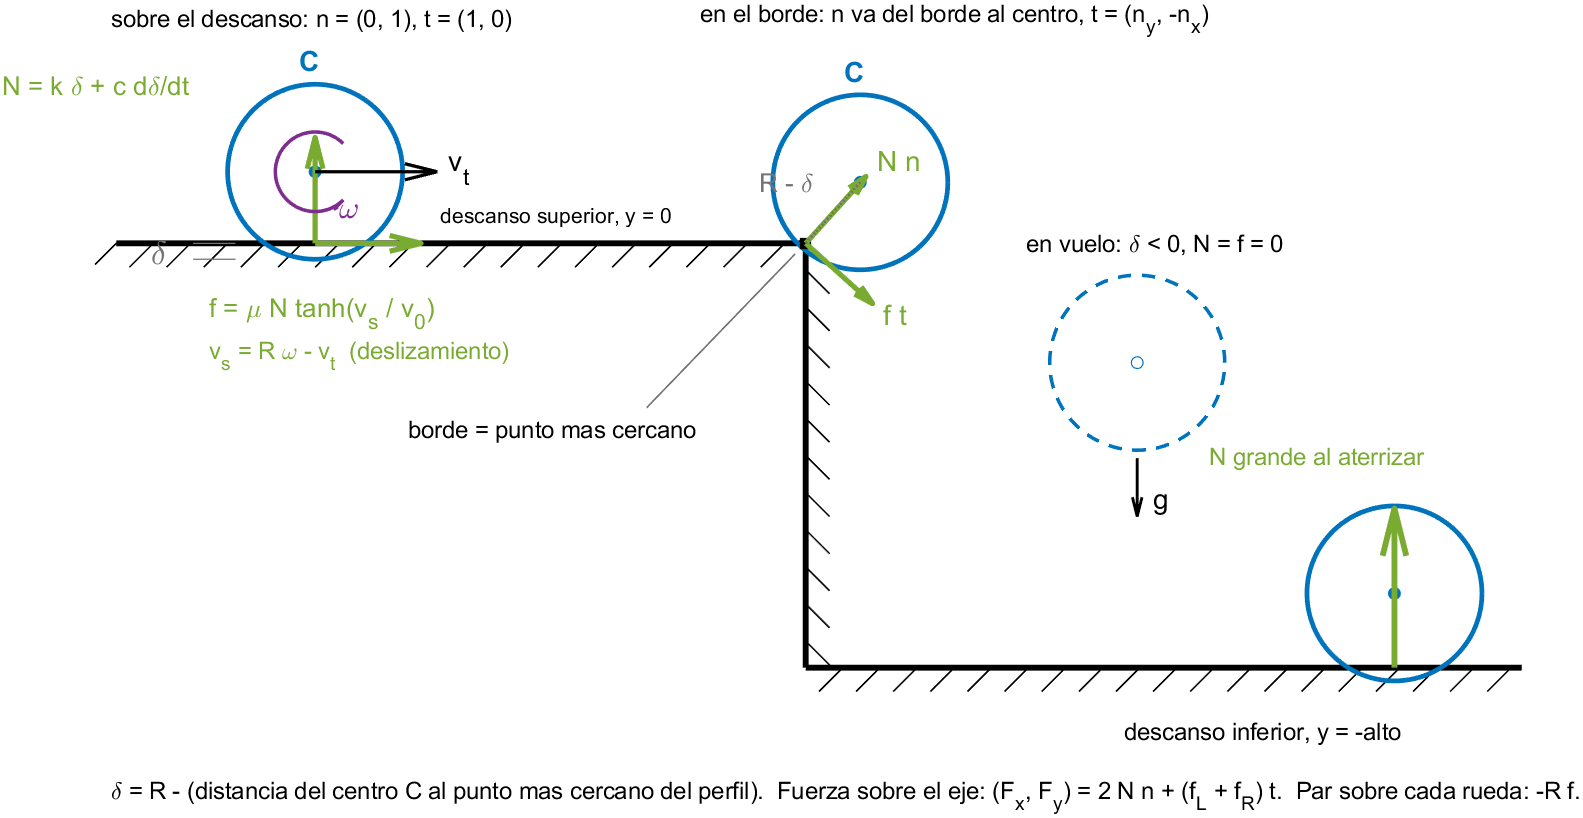
\includegraphics[width=0.95\textwidth]{fig_contacto}
  \caption{Contacto de la rueda con el perfil de escalones: sobre un descanso, en el borde, en vuelo y al
  aterrizar. $\delta$ está exagerada (en la realidad son décimas de milímetro).}
  \label{fig:contacto}
\end{figure}

El piso es un perfil de escalones descendentes: altura 0 para $x < x_0$, $-k\cdot alto$ en el descanso $k$
($k = 1..n$), con contrahuellas verticales en $x_0 + (k-1)\,ancho$; $n = 0$ es piso plano. Para el centro
de rueda $C = (x, y)$ se busca el punto más cercano del perfil (sobre los descansos, las contrahuellas o los
bordes) y se define
\begin{equation}
  \delta = R - |C - P_{cerc}|, \qquad \hat n = \frac{C - P_{cerc}}{|C - P_{cerc}|}, \qquad \hat t = (n_y,\ -n_x).
\end{equation}
Sobre un descanso $\hat n = (0,1)$; en un borde $\hat n$ es radial; contra una contrahuella es horizontal.
Si $\delta \le 0$ no hay contacto y la rueda está en vuelo. Si hay contacto, por rueda:
\begin{equation}
  N_i = \max\big(0,\ k_c\,\delta + c_c\,\dot\delta\big),\qquad \dot\delta = -\dot{\bm r}_w\cdot\hat n,
  \label{eq:N}
\end{equation}
\begin{equation}
  v_s = R\omega - \dot{\bm r}_w\cdot\hat t,\qquad f = \mu\,N_i\tanh(v_s/v_0) - c_v v_s .
  \label{eq:f}
\end{equation}
$k_c$ y $c_c$ son la rigidez y amortiguación del neumático; $v_s$ es la velocidad de deslizamiento (cero
si la rueda rueda sin patinar) y $\tanh$ suaviza la fricción de Coulomb: para $|v_s| \gg v_0$ la fuerza
satura en $\mu N_i$, para $|v_s| \ll v_0$ actúa como una rigidez viscosa alta que es lo que mantiene la
rodadura. La fuerza total sobre el eje y el par sobre cada rueda son
\begin{equation}
  (F_{cx}, F_{cy}) = 2N_i\,\hat n + (f_L + f_R)\,\hat t, \qquad \tau_{c} = -R f \ \ (\text{entra en \eqref{eq:rueda}}).
\end{equation}
En piso plano y en reposo, $N_i = k_c\delta_0 = m_{tot}g/2$: el neumático se hunde
$\delta_0 = m_{tot}g/(2k_c) \approx 0{,}17$\,mm.

\section{Servo y flexor}
\label{sec:flexor}

\textbf{Servo de hombro.} Tiene su propio lazo de posición. Se modela como par proporcional-derivativo al
error, saturado por su curva par--velocidad:
\begin{equation}
  \tau_s = \mathrm{sat}_{\pm\tau_{lim}}\big(K_p(\theta_{ref} - \theta) - K_d\dot\theta\big),\qquad
  \tau_{lim} = \begin{cases}\tau_{max}\,(1 - |\dot\theta|/\omega_{nl}) & \text{si el par impulsa el movimiento}\\ \tau_{max} & \text{si lo frena}\end{cases}
\end{equation}
con $\theta = \theta(l)$ y $\dot\theta = (\dd\theta/\dd l)\,\dot l$ de la tabla inversa, y
$F_{servo} = n_s\tau_s\,\dd\theta/\dd l$.

\begin{figure}[H]
  \centering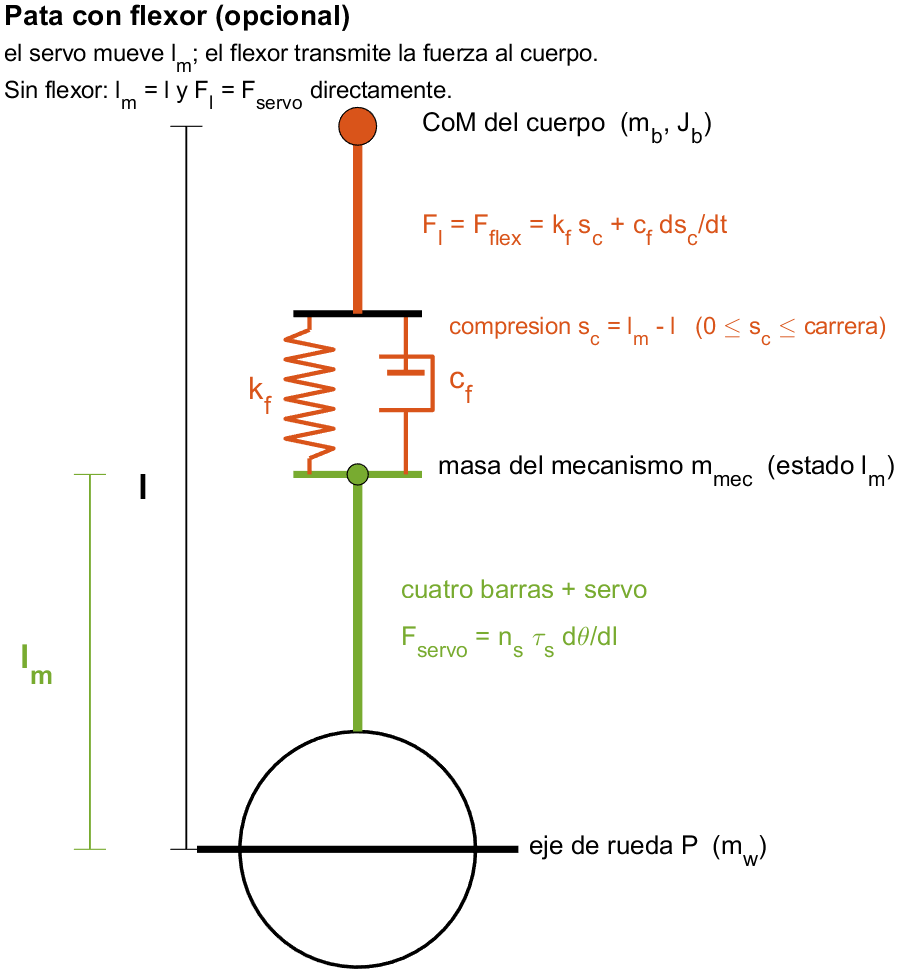
\includegraphics[width=0.6\textwidth]{fig_flexor}
  \caption{Pata con flexor: el cuatro barras impone $l_m$, el flexor (resorte $k_f$ y amortiguador $c_f$ en
  paralelo, con carrera limitada) transmite la fuerza al cuerpo.}
  \label{fig:flexor}
\end{figure}

\textbf{Flexor} (opcional, el del documento de dimensionamiento). Aparece un estado más, $l_m$, el largo que
impone el mecanismo, y la compresión $s_c = l_m - l$:
\begin{equation}
  F_{flex} = k_f s_c + c_f\dot s_c \ (+\ \text{topes si } s_c < 0 \text{ ó } s_c > carrera),\qquad
  m_{mec}\,\ddot l_m = F_{servo} - F_{flex} + f_{tope}(l_m) - b_l\dot l_m,
\end{equation}
y sobre el cuerpo entra $F_l = F_{flex}$. $m_{mec}$ es la masa de las barras, que es lo que el servo mueve.
Sin flexor, $F_l = F_{servo} + f_{tope}(l) - b_l\dot l$ directamente y $l_m$ no se usa.

\section{Estado completo e integración}

\begin{equation}
  X = [\,x,\ y,\ \phi,\ l,\ \dot x,\ \dot y,\ \dot\phi,\ \dot l,\ \theta_{wL},\ \omega_L,\ \theta_{wR},\ \omega_R,\ \theta_{mL},\ \omega_{mL},\ \theta_{mR},\ \omega_{mR},\ i_L,\ i_R,\ l_m,\ \dot l_m\,]
\end{equation}
Entradas $u = [V_L, V_R, \theta_{ref}]$, perturbaciones $d = [F_x, M_p, \alpha, \mu, F_{esc}]$. En cada
evaluación \code{robot\_planta} calcula, en este orden: tensión de bus y motores \eqref{eq:jeq}; contacto
\eqref{eq:N}--\eqref{eq:f}; servo y flexor; $M$, $C$, $G_v$ de \code{dinamica\_cuerpo\_gen}; el vector
\eqref{eq:Q}; $\ddot q = M^{-1}(Q - C - G_v)$; las aceleraciones de rueda \eqref{eq:rueda}; y la fuerza
específica en la IMU para los sensores. El integrador es \code{ode15s} (paso máximo 1\,ms, porque el
contacto es rígido) tanto en MATLAB como en Simulink.

\section{Modelo lineal para diseño}

Alrededor de la vertical, pata fija en $l_0$, rodadura sin deslizar ($\dot x = R\omega$, que elimina $f$ y mete
$J_{eq}$ en la masa), piso horizontal, estado $z = [x, \phi, \dot x, \dot\phi]$ y entrada el par total de
rueda $\tau_w$:
\begin{equation}
  M_2 = \begin{bmatrix} m_w + m_b + 2J_{eq}/R^2 & m_b l_0 \\ m_b l_0 & m_b l_0^2 + J_b \end{bmatrix},\qquad
  M_2\begin{bmatrix}\ddot x\\ \ddot\phi\end{bmatrix} = \begin{bmatrix} 0 \\ m_b g l_0\,\phi\end{bmatrix} - \begin{bmatrix} 2b_w/R^2 & 0 \\ 0 & b_\phi\end{bmatrix}\begin{bmatrix}\dot x\\ \dot\phi\end{bmatrix} + \begin{bmatrix} 1/R \\ -1\end{bmatrix}\tau_w,
\end{equation}
\begin{equation}
  A = \begin{bmatrix} 0 & I \\ -M_2^{-1}K_q & -M_2^{-1}D\end{bmatrix},\ K_q = \mathrm{diag}(0, -m_b g l_0),\qquad
  B = \begin{bmatrix} 0 \\ M_2^{-1}[1/R,\ -1]^T\end{bmatrix}.
\end{equation}
Polo inestable: $+8{,}0$\,rad/s (CAD, $l_0 = 134$\,mm) y $+10{,}3$\,rad/s (corregido, $l_0 = 121$\,mm); un
péndulo simple daría $\sqrt{g/l_0} \approx 8{,}6$ y $9{,}0$. Masa aparente $M_2(1,1)$: 12{,}1\,kg con 1:100
y 1{,}56\,kg con 1:21.

\section{Dónde está cada cosa en el código}

Todo está en \code{simulacion/planta\_v2/}. Se corre con \code{arrancar.m}; los tests, desde la raíz del
repositorio, con \code{runtests('simulacion/planta\_v2/tests')} (17 tests, todos pasan).

\begin{table}[H]
  \centering\footnotesize
  \begin{tabular}{>{\raggedright\arraybackslash}p{3.3cm} >{\raggedright\arraybackslash}p{5.4cm} >{\raggedright\arraybackslash}p{7.3cm}}
    \toprule
    Ecuación & Archivo & Qué hace \\
    \midrule
    \eqref{eq:D}--\eqref{eq:P} & \code{modelo\_base/cinematica\_pata.m} & directa: $\theta \to D, C, P, \mu_t$ (del zip del grupo) \\
    tabla $\theta \leftrightarrow l$, \eqref{eq:l} & \code{parametros\_robot.m} (bloque ``mapa'') & barre $\theta$, arma \code{P.tab.l}, \code{P.tab.th}, \code{P.tab.dthdl} \\
    interpolación & \code{interp\_lin.m} & lee la tabla (directa e inversa) \\
    \eqref{eq:T}--\eqref{eq:lag} & \code{derivar\_dinamica\_cuerpo.m} & Lagrange simbólico; genera \code{dinamica\_cuerpo\_gen.m} ($M$, $C$, $G_v$) \\
    \eqref{eq:Q}, \eqref{eq:rueda}, servo, flexor, IMU & \code{robot\_planta.m} & la planta completa: $\dot X = f(X, u, d, par)$ \\
    \eqref{eq:jeq} y reductor elástico & \code{motor\_reductor.m} & motor + reductor de un lado \\
    perfil, $\delta$, $\hat n$ & \code{perfil\_piso.m} & punto más cercano del piso de escalones \\
    \eqref{eq:N}--\eqref{eq:f} & \code{contacto\_rueda.m} & normal, fricción, fuerzas sobre el eje y pares \\
    modelo lineal & \code{modelo\_lineal\_robot.m} & $A$, $B$, $M_2$ en $l_0$ \\
    LQR & \code{disenar\_lqr\_robot.m} & ganancias $K(l)$ (control, otro informe) \\
    sensores / control & \code{robot\_sensores.m}, \code{robot\_controlador.m} & IMU, encoders, filtro, ley de control \\
    parámetros & \code{parametros\_editables.m} & \textbf{los valores que se editan} (sección~\ref{sec:param}) \\
    derivados & \code{parametros\_robot.m}, \code{parametros\_simulink.m} & convierte a SI, calcula $m_b$, $J_b$, CoM, tabla; arma \code{par} para Simulink \\
    ver lo que quedó & \code{mostrar\_parametros.m} & imprime todo en mm, g, kg\,cm \\
    escenarios & \code{escenarios\_robot.m}, \code{estado\_inicial.m} & condiciones iniciales, referencias, perturbaciones, escalones \\
    correr & \code{simular\_ode.m}, \code{simular\_slx.m}, \code{correr\_escenarios\_robot.m} & MATLAB puro, Simulink, barrido \\
    Simulink & \code{construir\_robot\_slx.m} & genera \code{robot\_segway.slx} \\
    \bottomrule
  \end{tabular}
  \caption{Mapa ecuación $\to$ código.}
\end{table}

Flujo de una corrida: \code{parametros\_robot} $\to$ \code{disenar\_lqr\_robot} $\to$ \code{escenarios\_robot}
$\to$ \code{simular\_ode} (o \code{simular\_slx}) $\to$ \code{resumen\_corrida} / \code{graficar\_corrida}.
En Simulink los tres bloques MATLAB Function (Robot/dinámica, Sensores, Controlador) llaman a las mismas
funciones y leen los parámetros de la estructura \code{par} del workspace.

\section{Qué puede cambiar el ingeniero, dónde y cómo}
\label{sec:param}

Todos los valores editables están en \textbf{un solo archivo}, \code{parametros\_editables.m}, agrupados
en 11 bloques, cada uno con su unidad, de dónde salió el valor y qué afecta. Nada más del código tiene
números del robot. Dos formas de cambiar algo:
\begin{enumerate}\itemsep2pt
  \item Editar el archivo y volver a correr (queda para todos).
  \item Sin editar, para probar: \code{P = parametros\_robot('corregido', 'mu', 0.4, 'm\_AD', 35);}
  Cualquier campo del archivo se puede pasar así por nombre.
\end{enumerate}
Después, \code{mostrar\_parametros(P)} imprime lo que quedó en unidades de ingeniería, incluidos los valores
derivados: $m_b$, $J_b$, posición del CoM, rango de $l$, $G$, par de servo necesario, masa aparente por el
rotor reflejado, hundimiento del neumático.

\begin{table}[H]
  \centering\scriptsize
  \begin{tabularx}{\textwidth}{>{\raggedright\arraybackslash}p{2.3cm} >{\raggedright\arraybackslash}p{4.3cm} >{\raggedright\arraybackslash}p{1.9cm} >{\raggedright\arraybackslash}p{2.0cm} X}
    \toprule
    Qué & Nombre en \code{parametros\_editables} & Unidad & Valor actual & Cómo se obtiene / qué afecta \\
    \midrule
    \multicolumn{5}{l}{\textbf{Masas (pesar las piezas impresas y reemplazar)}} \\
    manivela, balancín, acoplador & \code{m\_AD}, \code{m\_BC}, \code{m\_CDP} & g por pata & 29, 7, 19.5 & balanza; entran a $m_b$, CoM y $J_b$ \\
    cabina, tapa & \code{m\_cabina}, \code{m\_tapa} & g & 207, 114 & balanza; dominan $m_b$ y $J_b$ \\
    batería, electrónica, tornillería & \code{m\_bateria}, \code{m\_electronica}, \code{m\_tornilleria} & g & 120, 60, 50 & balanza; con su posición \code{r\_*} respecto de $A$ \\
    carga extra & \code{m\_carga}, \code{r\_carga} & g, mm & 0 & lo que se le cuelgue a la cabina \\
    rueda, motor & \code{m\_rueda}, \code{m\_motor} & g cada uno & 30, 95 & balanza; forman $m_w$ \\
    \multicolumn{5}{l}{\textbf{Inercias}} \\
    del cuerpo & \code{J\_cuerpo} & kg\,m$^2$ & \code{[]} (calculada) & \code{[]} la calcula de las piezas por Steiner; un número la impone (p.\,ej. medida con péndulo bifilar) \\
    de cada pieza & \code{J\_cabina}, \code{J\_tapa}, \code{J\_AD}, \ldots & kg\,m$^2$ & del STEP & sólo si cambia la pieza \\
    de la rueda & \code{J\_rueda} & kg\,m$^2$ & \code{[]} = disco & \code{[]} usa $\tfrac12 m R^2$ \\
    del rotor & \code{J\_r} & kg\,m$^2$ & $6\cdot10^{-7}$ & hoja del motor; se refleja $\times n_g^2$ \\
    \multicolumn{5}{l}{\textbf{Rigideces y amortiguaciones}} \\
    neumático & \code{k\_contacto}, \code{c\_contacto} & N/m, N\,s/m & 30\,000, 60 & apretar la rueda con peso conocido y medir; fija el pico de impacto \\
    flexor & \code{flexor}, \code{k\_flexor}, \code{c\_flexor}, \code{carrera\_flexor} & --, N/m, N\,s/m, mm & off, 1080, 8, 40 & ensayo de flecha del flexor (docx) \\
    reductor & \code{gear\_rigido}, \code{k\_g}, \code{c\_g}, \code{juego\_deg} & --, N\,m/rad, N\,m\,s/rad, ° & rígido, 50, 0.05, 1.5 & sólo si se activa el eje elástico \\
    topes de carrera & \code{k\_tope}, \code{c\_tope} & N/m, N\,s/m & 20\,000, 60 & numéricos; no tocar salvo que la ODE se ponga lenta \\
    \multicolumn{5}{l}{\textbf{Fricción}} \\
    rueda--piso & \code{mu} & -- & 0.7 & goma sobre madera 0.7, baldosa lisa 0.4; se puede variar en el tiempo desde el escenario \\
    suavizado de Coulomb & \code{v\_s}, \code{c\_v} & m/s, N\,s/m & 0.005, 0.5 & numéricos \\
    eje de rueda, cabeceo, pata & \code{b\_w}, \code{b\_pitch}, \code{b\_pata} & N\,m\,s/rad, N\,m\,s/rad, N\,s/m & $10^{-4}$, $10^{-3}$, 8 & supuestos chicos; medir por decaimiento \\
    \multicolumn{5}{l}{\textbf{Geometría}} \\
    bancada & \code{AB}, \code{ang\_AB} & mm, ° & 80 / 47.5 ó 100 / 45 & según variante; agujeros de la cabina \\
    barras & \code{s\_barras}, \code{k\_AD} \ldots & mm, -- & 100; 1.4, 1.35, 0.51, 1.4 & si se reimprimen a otra escala \\
    rueda & \code{Rw} & mm & 33 & radio; cambia velocidad, par y altura \\
    escalones & \code{piso\_x0}, \code{piso\_alto}, \code{piso\_ancho}, \code{piso\_n} & m, m, m, -- & 0.5, 0.16, 0.30, 0 & los escenarios fijan \code{piso\_n} \\
    \multicolumn{5}{l}{\textbf{Motor, batería, servo}} \\
    motor & \code{R\_m}, \code{L\_m}, \code{w\_nl\_motor\_rpm}, \code{N}, \code{tau\_c}, \code{b\_m} & $\Omega$, H, rpm, --, N\,m, N\,m\,s/rad & 5.45, 1.5e-3, 6000, 100 ó 21.3 & hoja de datos del motor comprado \\
    batería & \code{V\_bat}, \code{R\_bat} & V, $\Omega$ & 11.1, 0.05 & medir en carga \\
    servo & \code{tau\_s\_max}, \code{w\_nl\_servo}, \code{Kp\_s}, \code{Kd\_s} & N\,m, rad/s, N\,m/rad, N\,m\,s/rad & 2.4, 7.7, 45, 1 & hoja de datos a la tensión real \\
    \multicolumn{5}{l}{\textbf{Sensores y control}} \\
    período, retardo & \code{Ts}, \code{n\_delay} & s, muestras & 0.005, 1 & del firmware \\
    IMU & \code{d\_imu}, \code{gyro\_bias\_dps}, \code{gyro\_rms\_dps}, \code{acc\_rms\_g} & mm, °/s, °/s, g & (-18.5, 21), 0.5, 0.1, 0.02 & posición en la cabina; hoja del MPU6050 \\
    encoder & \code{encoder}, \code{CPR\_motor} & --, pulsos & true, 11 & del motor -371 \\
    \bottomrule
  \end{tabularx}
  \caption{Parámetros editables. Los marcados como ``numéricos'' regulan la integración, no la física.}
\end{table}

\paragraph{Ejemplos.}
\begin{itemize}\itemsep2pt
  \item \emph{Pesaron las piezas impresas}: AD dio 35\,g, CDP 24\,g, cabina 230\,g. Editar \code{m\_AD = 35},
  \code{m\_CDP = 24}, \code{m\_cabina = 230}; correr \code{P = parametros\_robot('corregido'); mostrar\_parametros(P)}
  y ver el nuevo $m_b$, $J_b$ y el par de servo necesario. El LQR se rediseña solo al correr \code{arrancar}.
  \item \emph{Midieron la inercia del cuerpo} colgándolo como péndulo: $J_b = 3{,}5\cdot10^{-3}$\,kg\,m$^2$.
  Poner \code{J\_cuerpo = 3.5e-3}; \code{mostrar\_parametros} avisa ``IMPUESTA''.
  \item \emph{Piso resbaloso}: \code{mu = 0.4}, o sólo para una corrida
  \code{parametros\_robot('corregido','mu',0.4)}. El escenario \code{resbaloso} además lo cambia en el tiempo.
  \item \emph{Otro motor} (JGB37-520 de 319\,rpm): cargar \code{R\_m}, \code{w\_nl\_motor\_rpm}, \code{N} y
  \code{J\_r} de su hoja de datos en el bloque 7. El par de bloqueo y la masa aparente que imprime
  \code{mostrar\_parametros} dicen enseguida si conviene.
  \item \emph{Midieron el neumático}: 20\,N lo aplastan 0{,}8\,mm $\Rightarrow$ \code{k\_contacto = 25000}.
\end{itemize}

\section{Hipótesis a revisar}

\begin{itemize}\itemsep2pt
  \item Barras como parte del cuerpo (CoM e inercia promediados sobre $\theta$); no se modela la inercia del
  cuatro barras alrededor del hombro.
  \item El desvío horizontal de $P$ se absorbe en $\phi$: hasta 4° de cabina inclinada en equilibrio con el CAD actual.
  \item Patas sincronizadas, sin guiñada ni asimetrías.
  \item Contacto Coulomb suavizado, neumático lineal; sin deformación de la rueda más allá de $k_c$.
  \item Reductor rígido por defecto; juego y elasticidad con valores supuestos.
  \item Motor de 60\,rpm extrapolado de la variante de 350\,rpm; $J_r$ típico.
  \item Servo como lazo proporcional-derivativo con límites de hoja de datos.
  \item Masas impresas con densidad efectiva supuesta: pesar.
\end{itemize}
\end{document}
